\documentclass[conference]{IEEEtran}
\IEEEoverridecommandlockouts
% The preceding line is only needed to identify funding in the first footnote. If that is unneeded, please comment it out.
\usepackage{cite}
\usepackage{amsmath,amssymb,amsfonts}
\usepackage{algorithmicx}
\usepackage{graphicx}
\usepackage{textcomp}
\usepackage{xcolor}
\usepackage[numbers]{natbib} 
\usepackage{algorithm}
\usepackage{algpseudocode}
\usepackage{multirow}
\usepackage{pifont}
\newcommand{\cmark}{\ding{51}}%
\newcommand{\xmark}{\ding{55}}%
\def\BibTeX{{\rm B\kern-.05em{\sc i\kern-.025em b}\kern-.08em
    T\kern-.1667em\lower.7ex\hbox{E}\kern-.125emX}}
\begin{document}

\title{Improved Bug Localization using Keyword-Source Co-occurrence\\
%{\footnotesize \textsuperscript{*}Note: Sub-titles are not captured in Xplore and
%should not be used}
\thanks{Identify applicable funding agency here. If none, delete this.}
}

\author{\IEEEauthorblockN{Shamima Yeasmin~~~Mohammad Masudur Rahman~~~Chanchal K. Roy~~~ Kevin A. Schneider}
\IEEEauthorblockA{\textit{Department of Computer Science} \\
\textit{ University of Saskatchewan}\\
Saskatoon, Canada \\
shy942@mail.usask.ca, \{masud.rahman, chanchal.roy, kevin.schneider\}@usask.ca}
%\and
%\IEEEauthorblockN{Mohammad Masudur Rahman}
%\IEEEauthorblockA{\textit{dept. name of organization (of Aff.)} \\
%\textit{name of organization (of Aff.)}\\
%City, Country \\
%email address}
%\and
%\IEEEauthorblockN{Chanchal K. roy}
%\IEEEauthorblockA{\textit{dept. name of organization (of Aff.)} \\
%\textit{name of organization (of Aff.)}\\
%City, Country \\
%email address}
%\and
%\IEEEauthorblockN{Kevin A. Schneider}
%\IEEEauthorblockA{\textit{dept. name of organization (of Aff.)} \\
%\textit{name of organization (of Aff.)}\\
%City, Country \\
%email address}

}

\maketitle

\begin{abstract}
Bug localization is one of the most challending tasks undertaken by the developers during software maintenance.
Existing studies mostly rely on lexical similarity between the bug reports and source code for bug localization.
However, such similarity always does not exist, and these studies suffer from vocabulary mismatch issues.
In this paper, we propose a bug localization technique that (1) not only uses lexical similarity between bug report and source code documents  
but also (2) exploits the co-occurrences between keywords from the past reports and source links from corresponding changed code.
Experiments using a collection of ~6000 bug reports show that our technique can locate buggy files with a Top-10 accuracy of 62.14\% and a mean reciprocal rank@10 of 0.50 and a mean precision average@10 of 70\%, which are highly promising. 
Comparison with state-of-the-art IR-based bug localization techniques confirms superiority of our technique. 
\end{abstract}

\begin{IEEEkeywords}
bug localization, bug report, source codes, association map
\end{IEEEkeywords}

\section{Introduction}
Bug localization is the process of locating the source codes that need to be changed in order to fix a given bug. 
Locating buggy files is time-consuming and costly if it is done by manual effort, especially for the large software system when the number of bug of that system becomes large. Therefore, effecting methods for locating bugs automatically from bug reports are highly desirable. 
In automatic bug localization technique, it takes a subject system as an input and produces a list of entities such as classes, methods etc. against a search query. For example, information retrieval based techniques rank the list of entities by predicted relevance and return a ranked list of entities or source codes which may contain the bug. 
The bug localization techniques are also affected by the fact of designing effective query. If a query contains inadequate information, then the retrieval results will not be relevant at all. One other thing that the performance of existing bug localization approach did not reach to an accepted level and so far those studies showed good results for a small set of bugs. Therefore,
%However, static bug localization technique has an advantage over dynamic technique, as it does not require any working subject system rather it can apply on any stage of a system. 
in this paper, we apply a bug localization technique on large dataset that exploits an association link established from bug report repository to source code base through commit logs. 

In existing studies, information retrieval techniques  \cite{Jian} \cite{Saha} \cite{Moreno} \cite{Anh} \cite{Lukins} are applied to automatically search for relevant files based on bug reports.
In one case of Text Retrieval (TR) based approaches, \citet{Jian} propose BugLocator using revised Vector Space Model (rVSM), which requires the information extracted from bug reports and source codes. One of the issue association with TR-based technique is treating source codes as flat text that lacks structure. But exploiting source code structure can be a useful way to improve bug localization accuracy.
Due to the fuzzy nature of information retrieval, textually matching bug reports against source
files may have to concede noise (less relevant but accidentally matched words). However, large files are more
likely to contain noise as usually only a small part
of a large file is relevant to the bug report. So, by treating
files as single units or favoring large files, the techniques are more
likely to be affected by the noise in large files. So, \citet{Saha} present BLUiR, which retrieve structural information from code constructs.
However, bug reports often contain stack-trace information, which may provide direct clues for possible faulty files. Most existing approaches directly treat the bug descriptions as plain texts and do not explicitly consider stack-trace information. Here, \citet{Moreno} combine both stack trace similarity and textual similarity to retrieve potential code elements. 
To deal with two issues associated with source code structure and stack trace information, 
\citet{Chu}  proposed  a technique that use segmentation i.e., divides each source code file into segments and use stack-trace analysis, which significantly improve the performance of BugLocator.

LDA topic-based approaches \cite{Anh} \cite{Lukins} assume that the textual contents of a bug report and it's corresponding buggy source files share some technical aspects of the system.
Therefore, they develop topic model that represents those technical aspects as topic. 
However, existing bug localization approaches applied on small-scale data for evaluation so far.
Besides the problem of small-scale evaluations, the performance of the existing bug localization methods can be further improved too. For example, using Latent Dirichlet Allocation (LDA), only buggy files for 22\% of Eclipse 3.1 bug reports are ranked in the top 10 [25]. 
But, now it is an important research question to know how effective these approaches are for locating bugs in large-scale (i.e., big data).
In the field of query processing
\citet{Sisman}  proposed a method that examines the files retrieved for the initial query supplied by a user and then selects from these files only those additional terms that are in close proximity to the terms in the initial query. Their \cite{Sisman} experimental evaluation on two large software projects using more than 4,000 queries showed that the proposed approach leads to significant improvements for bug localization and outperforms the well-known QR methods
in the literature.
There are two common issues associated with existing studies. First, 
most of the bug localization techniques exploit lexical similarity measure for retrieving relevant files from the code base. So, it is expected that the search query constricted from new bug report should contain keywords similar to code constructs in code base. This issue demands developers or users  previous expertise on the given project, which can not be guaranteed in real world. 
Second, closely related to the first issue there is another well known problem called vocabulary mismatch. In order to convey the same concept on both search query (i.e., new bug report) and source code files the developers tend to use different vocabularies. This issue questions the applicability of exploiting lexical similarity measure.

So, in order to resolve these two issues, in our work we propose a bug localization approach that combines lexical similaority with word co-occurrence measue. 
Our proposed technique exploits the association of keywords extracted from fixed bug report with their changed source code location. Here, the main idea is to capture information from a collection of bug reports and exploit them for locating relevant source code location.
So our approach not (1) only relies on the lexical similarity measure between big reports and source code files for bug localization, and (2) but also addresses the vocabulary mismatch problem by using a keyword-source map constructed from fixed bug information.

We also replicate two state of the art bug localization techniques in order to compare the performance of our proposed approach with these two.

\section{An Example Use Case Scenario}\label{sec:usecase}
\begin{table*}[t]
	\centering
	\caption{A working example of BLuAMIR}
	\label{tab:workingexample}
	\resizebox{6.0in}{!}{%
		\begin{tabular}{c|c|c||c|c|c|c|c|c}
			\hline
			%\begin{tabular}[c]{@{}c@{}}\#Bugs for \\ developing \\ map databases\end{tabular} &
			\textbf{Query \#ID}
			& \textbf{VSM score}  
			& \textbf{Retrieved Files}  & 
			\textbf{GoldSet}  &
			\textbf{VSM score}  & 
			\textbf{Co-Occ-Score} &
			\textbf{ScoreAll} &
			\textbf{Retrieved Files} &
			\textbf{Goldset}\\
			\hline
		    \multirow{10}{*}{37026} & 1.00 & WorkingSetLabelProvider.java  & \checkmark &  &  & 0.85 & WorkingSetLabelProvider.java & \checkmark \\
			\cline{2-9}
		    & 0.80 & ImageFactory.java & \xmark & & & 0.69 & WorkingSet.java & \checkmark \\ 
		  \cline{2-9}
		   & 0.76 & WorkingSetMenuContributionItem.java & \xmark & & & 0.67 & IWorkingSet.java.java & \checkmark\\
		   \cline{2-9}
		   & 0.75 & IWorkingSet.java & \checkmark & & & 0.64 & WorkingSetTypePage.java & \xmark\\
		  \cline{2-9}
		   & 0.70 & ProjectImageRegistry.java & \xmark & & & 0.63 & CommandImageService.java & \xmark \\
		   \cline{2-9}
		   & 0.68 & IWorkingSetManagerTest.java & \xmark & & & 0.61 & WorkbenchImages.java & \checkmark\\
		   \cline{2-9}
		   & 0.67 & IWorkbenchPartDescriptor.java & \xmark & & & 0.60 & WorkingSetAdapterFactory.java & \checkmark \\
		   \cline{2-9}
		   & 0.65 & MockWorkingSetPage.java & \xmark  & & & 0.57 & EditorIconTest.java & \xmark\\
		 \cline{2-9}
		   & 0.65 & MissingImageDescriptor.java & \xmark  & & & 0.57 & PerspectiveDescriptor.java & \xmark \\
		  \cline{2-9}
		   & 0.64 & WorkingSetTypePage.java & \xmark & & & 0.56 & IAction.java & \xmark\\
		   \hline
	\end{tabular}}
	\centering
\end{table*}
Note:
Provide an example such as say for bug B1 source code files F1, F2, F3 are modified or changed. Now a new bug B has similar to B1 in terms of cosine similarity. Then prove that F1, F2, F3 or one or two of them are contained in the list of files which would be changed or modified for fixing that new bug B.
Lets consider a bug having ID "" from Eclipse-UI-Platform software. From Git repository it is discoverd that so far n number of file have been modified in order to fix this bug. We also csn find the source code address of those changed files. Now, 

In another example, show that the words or keywords of a bug B are aslo presented in the source code files F1, F2 or F3. 

\section{Existing Approaches}\label{sec:existing}
We have replicated two existing bug localization approaches: (i) TF-IDF based bug localization approach and (ii) LDA topic based bug localization technique. In the following subsections we will briefly discuss each of them.
\subsection{TF-IDF Based Bug Localization Technique:}
In this technique, each source code file is ranked based on source code file scores and similar bugs information. Source code file contains words those can be also occurred in the bug reports. This is considered as a hint to locate buggy files. If a new bug is similar to a given previously located bug, then there is a possibility that the source code files located for the past bug can provide useful information in finding buggy files for that new bug. Based on these two assumptions, we compute scores for all source code files for a given project. However, we need to focus on some concepts which are required to understand the  system. They are described as follows:

\textbf{Ranking based on TF-IDF calculation:}
The basic idea of a TF-IDF model is that the weight of a term in a document is increasing with its occurrence frequency in this specific document and decreasing with its occurrence frequency in other documents \cite{Jian}.
In this approach we have used a revised Vector Space Model (rVSM) proposed by \citet{Jian} in order to index and rank source code files. 
The main difference between classic VSM and revised VSM is that in case of revised version logarithm variant is used in computing term frequency. The equation is:
\begin{equation}
tf(t+d)=log(f_{td})+1
\end{equation}
Here \textit{tf} is the term frequency of each unique term \textit{t} in a document \textit{d} and \textit{f\textsubscript{td}} is the number of times term \textit{t} appears in document \textit{d}.
So the new equation of revised VSM model is as follows:

\begin{multline}\label{rVSMequation}
rVSMScore(q,d)=g(\#term)\times cos(q,d)
\\
\frac{1}{1+e^{-N(\#terms))}}\times \frac{1}{\sqrt{\sum_{t\epsilon q}}((logf_{tq}+1)\times log(\frac{\#docs}{n_{t}}))^{^{2}}}\times 
\\
\frac{1}{\sqrt{\sum_{t\epsilon d}((log {f_{td}+1})\times log(\frac{\#docs}{n_{t}}))^{2}}}\times
\\
\sum_{t\epsilon q\bigcap d}(logf_{tq}+1)\times (logf_{td}+1)\times log(\frac{\#docs}{n_{t}})^{2}
\end{multline}
%\end{equation}
This \textit{rVSM} score is calculated for each query bug report \textit{q} against every document \textit{d} in the corpus. However, in the above equation \textit{\#terms} refers to the total number of terms in a corpus, \textit{n\textsubscript{t}} is the number of documents where term \textit{t} occurs.

\textbf{Ranking based on similar bug information}
\begin{figure}
	\centering
	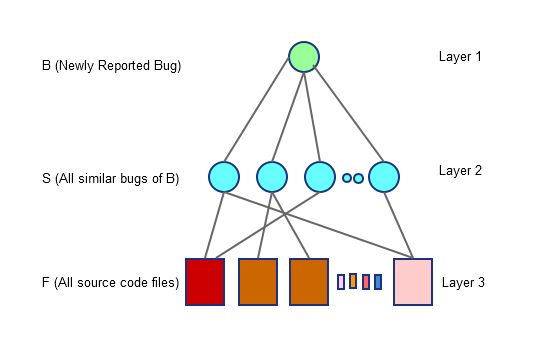
\includegraphics[scale=0.65]{3layers}
	\caption{Bug and its Similar Bug Relationship with Source Code Files:}
	\label{fig:BSBR}
\end{figure}
The assumption of this ranking is similar bugs of a given bug tend to modify similar source code files. Here, we construct a 3-layer architecture as described in \cite{Jian}. In the top layer (layer 1) there is a bug \textit{B} which represents a newly reported bug. All previously fixed bug reports which have non-negative similarity with bug  \textit{B} are presented in second layer. In third layer all source code files are shown. In order to resolve each bug in second layer some files in the corpus were modified or changed, which are indicated by a link between layer 2 and layer 3. Foe all source code files in layer 3, similarity score is computed, which can be referred to as degree of similarity. The score can be defined as:

\begin{equation}\label{Simiequation}
SimiScore=\sum_{All S_{i} that connect to F_{j}}(Similarity(B,S_{i})/n_{i})
\end{equation} 
Here, similarity between newly reported bug \textit{B} and previously fixed bug \textit{S\textsubscript{i}} is calculated based on cosine similarity measure and \textit{n\textsubscript{i}} is the total number of link \textit{S\textsubscript{i}} has with source code files in layer 3.

%\subsection
\textbf{Combining Both Ranks:}
We combine the both scores based on source code score and similar bugs score as in \cite{Jian} as follows:
\begin{equation}
FinalScore=(1-\alpha )\times N(rVSMScore)+\alpha \times N(SimiScore)
\end{equation}

\subsection{LDA Topic Based Bug Localization Technique:}
The main assumption behind this technique is the textual content of the bug reports and their associated buggy source code files tend to describe some common technical aspects. So, if  we could identify the technical topics extracted from both bug reports and source codes, we could recommend the files shared technical topics with the newly reported bug reports. If a newly reported bug has similar technical topics with some previously fixed bug reports, the fixed files could be a good candidate files for newly reported bug.

LDA (Latent Dirichlet Allocation) is a probabilistic and fully generative topic model. It is used to extract latent (i.e., hidden) topics, which are presented in a collection of documents. It also model each document as a finite mixture over the set of topics [add link here]. In LDA, similarity between a document \textit{d} and a query \textit{q} is computed as the conditional probability of the query given that document \cite{Lukins2}.

\begin{equation}
Sim(q,d_{i})=P(q|d_{i})=\prod_{q_{k}\epsilon q}P(q_{k}|d_{i})
\end{equation}

Here \textit{q\textsubscript{k}} is the \textit{k}th word in the query {q} Thus, a document (i.e., source code file) is relevant to a query if it has a high probability of generating the words in the query.

We perform the following steps in order to localize buggy files for newly reported bug using LDA based approach:

\begin{itemize}
	\item Apply topic modeling on the source code files. The output contains a certain number of topics and some associated keywords for each topic. We also get some other distribution files such as document-topic, word-topic etc.
	\item Now work with the documents topic distribution file. Make a list of source code documents or files for each topic. So, we wiill have a list that contain all topics and their associated source code documents.
	\item Here our query is the newly reported bug. This contains information in the bug reports such as title and short description etc. We all do inference for this query using a topic modeling tool. It will extract all topic associated with the query (i.e., newly reported bug).
	\item Now we need to work with topic keywords. We are going to perform a comparison between newly reported bug or the given query and source code files using topic information. That means we will compare topic-keywords associated with topics inferred for the query with topic-keywords of each topic extracted from source code documents.
	\item We will rank them based on topic-keyword similarity. So, now we know which are the top most topics, and we already have information regarding topic-document relationship, we will retrieve all source code files associated with all those top most topic as recommended buggy files.
	%\item A detailed description of methodologies for visualizing topic evolution extracted from bug reports.
	%\item A detailed description of methodologies for visualizing bug report extractive summaries.
	%\item Evaluation of visualized bug report extractive summary by conducting a task-oriented user study.
\end{itemize}
\section{Proposed System Diagram}\label{sec:proposedsystemDiagram}
Our proposed approach combine lexical similarity and co-occurence similarity measure.  \citet{Jian} proposed BugLocator based on two different similarity scores- one is rVSM score and the other one is Simi score. In our porposed bug localization approach, we retrieve relevant ranked files based on three different scores- 1) rVSM, 2) Simi and 3) Word Co-occurence. So,
we have divided our approach into two different sections or parts- 1) calculate rVSM and Simi scores and co-occurence measure and 2) combine all three scores in order to localize recommended buggy source files for a given newly reported bug. As we have combined two existing scores with our proposed word co-occirence score, we will discuss the system diagram of association map database in Part I and then we represent our overall system diagram in Part II.

\subsection{Part I: Mapping Bug Source Code Links}
In Part I, we construct an association map database - between keywords extracted from previously fixed bug reports collection and source code links. The system diagram for Part I is given in Fig. \ref{fig:MP}.

This mapping construction involves two steps.
At first we create association map using information contained in bug reports collection and commit logs. We collect information from title and description fields of each bug report. There are also developers comment section in a bug report, which is highly informative. But large documents also tend to reduce performance by taking too long to process. So, we reluctant to include developers comments of each bug report. However, we extract keywords from each bug report after preprocessing them such as stop word removal. 
%In this part, information are collected from bug report, version repository and source code repository. 
In version repository, we have commit logs, where the developers commit for several changes in a software project. For example, when a bug report is fixed, the developer who fixed this bug also creates a commit log containing which type of change he had to made to resolve the bug associated with the location of the source code files where the change has made. So, if we analyze commit logs, we can retrieve source code files information which have been changed in order to fix a given bug. Here the idea is, we first extract keywords from bug report and source code links for the same bug from commit log and then construct an association map database containing this mapping information. The links between keywords and source code links can be described as: each or several keywords can be linked to one or more source code links and each source code link can be linked to one or several keywords. This way we connect keywords and source code links to form an association map database named keyword-source code links. 

\begin{figure}
	\centering
	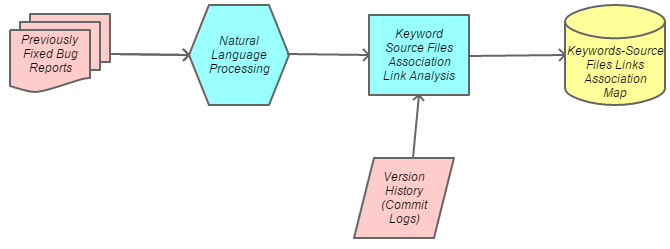
\includegraphics[scale=0.55]{Map}
	\caption{Proposed System Diagram: Mapping}
	\label{fig:MP}
\end{figure}


\begin{figure*}
	\centering
	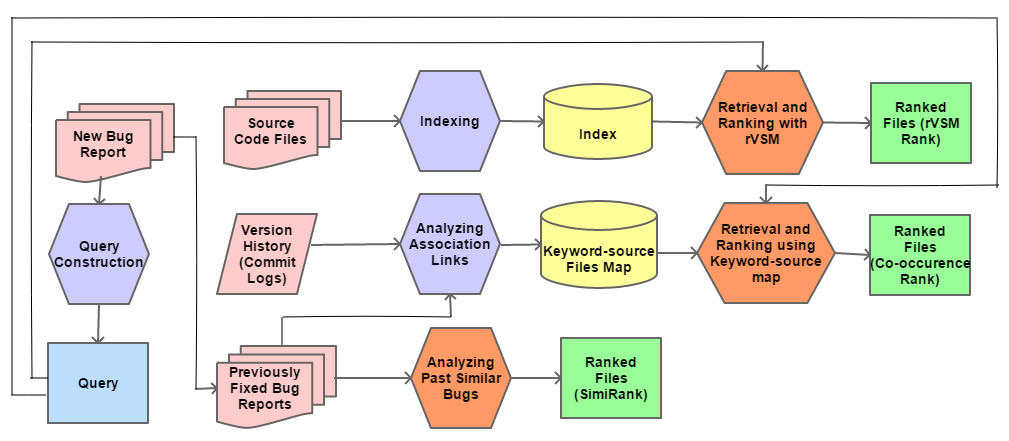
\includegraphics[scale=0.75]{SD1}
	\caption{Proposed System Diagram: Bug Localization}
	\label{fig:BL}
\end{figure*}

\subsection{Part II: Bug Localization Using rVSM, and Co-occurence Ranks}

The system diagram for this part has illustrated in Fig. \ref{fig:BL}.
In our system, we have three different ranks i.e., rVSM, Simi and Co-occurence. We utlize an existing technique proposed by \citet{Jian} for computing rVSM and Similarity scores. Basically, rVSM is a TF-IDF based score, which is measured between query and source code files.
On the other hand, Simi score refers to that fact that if a bug is similar to another bug, then they both tend to relate to same sources. However, we describe both scores in Section \ref{sec:existing}.
We have constructed an association map databases from keywords collected from bug report to its source code location information in Section \ref{sec:proposedsystemDiagram}.
For the candidate keyword tokens for the initial query, we exploit association map database (i.e., keyword-source code links) and retrieve the relevant source code files. We use some heuristic functions in order to combine three ranks and recommend buggy relevant source files. 


\section{Proposed Approach}\label{sec:proposedApproach}
Our proposed approach consists of two parts - (i) constructing association map databases and (ii) retrieve relevant buggy source code files. 

\subsection{Construction of Association Map Database Between Bug Reports and Source Files}
In this part, we construct two association map databases - one is between keywords and source code links extracted from bug reports and commit messages respectively and other one is between source code links and code token extracted from commit messages and source code content respectively. This section can be further divided into several parts: keyword extraction from bug reports, source code link extraction from commit logs, keyword- source code linking, code tokens extraction from source codes and source code-code token linking. They are discussed in the followings:

\begin{algorithm}[!t]
	\caption{Construction of Association Map Database Between Bug Reports and Source Files}
	\label{map}
	\begin{algorithmic}[1]
		\Procedure{BUG REPORTS }{$BRC$}\Comment{$BRC$: a collection of bug reports}
		\State $MAP_{KS} \gets$ \{\}\Comment{an association map}
		\Comment{creating adjacency map database from the bug reports collection}
		\State $MAP_{adj} \gets$ createAdjacencyDatabase($BRC$)
		\Comment{creating a map that links keywords into their bug ids}
		\State $MAP_{kb} \gets$ createKeywordsToBugMaps($MAP_{adj}$)
		\Comment{collecting unique keywords from keywords to bug map}
		
		%\LineComment{preprocess the collected keywords}
		%\For{Keyword $K_i \in$ $K$}
		\State $KB \gets$ collectKeywords($MAP_{kb}$)
		
		\Comment{Linking keywords from a bug report into its change set files}
		\For{keywords $KB_{_i}$ $\in$ $KB$}
		\State $BUG_{id} \gets$ retrieveBugIds ($K_i$)
		\For{each bug id $BUG_{id_j} \in BUG_{id}$}
		\State $SF_{links} \gets$ getLinkedSourceFiles($BUG_{id}$)
		\Comment{maps all source code files to its keywords}
		%\State $MAO_{BUG_{id}} \gets$ linkSourceCodeFiles$Adj_{T_i}, Adj_{K_j}$) 
		\State $MAP[KB_i].links \gets MAP[KB_{i}].links + SF_{links}$
		\EndFor
		\EndFor
		
		\Comment{collecting all keyword-source files links}
		\State $MAP_{KS} \gets$ $MAP[KB]$ 
		%\LineComment{put them into map}
		%\State $MAP \gets$ mapping()
		\State \textbf{return} $MAP_{KS}$
		\EndProcedure
	\end{algorithmic}
\end{algorithm}



\textbf{Keyword Extraction from Bug Reports:} We collect title, description and developers comments from each fixed bug report in a collection of bug reports. We perform standard natural language pre-processing on the corpus such as stop word removal, splitting and stemming. The purpose of removing stop words is that they contain very little semantic for a sentence. The process of stemming step extracts the root of each of the word. We use this stop word list [link] during stop word removal and this stemmer [link]for stemming. 

\textbf{Source Code Link Extraction from Commit Logs:}
We go through all commit messages and try to find those commit message that contain keywords related to bug fix such as fix, fixed and so on. Each of these commit messages presents other information such as the ID of bug report for which it was created and the links of the changed source code files. We then construct a relationship against each fixed bug report ID into their changed source code files links.

\textbf{Keyword- Source Code Linking:}
At this point, in one side we have pre-processed keywords associated with each bug report and on the other side we have a relationship information between bug report ID and buggy source code links. We construct a bipartite graph between keywords collected from a bug report to its buggy source code locations. Here, one or more keywords can be linked to one or more buggy source code files links and a source code file link can be linked to one or more keywords.

\textbf{Calculating Co-occurence Scores}
A query typically contains several keywords or words. For each keyword, we look for relevant source files in the keyword-source files association map. We assume these files are relevant because we created the map between the content of bug reports and their buggy source files. However, when we analysis these links for all keywords in a query, a relevant file can be found more than once. So we normalize the frequency of source files using standard TFIDF normalization technique. Then we recommend first Top-K files with their CoOccScores. The equation for computing co-occurence score is given belows:
\begin{equation}\label{CoOccequation}
SimiScore=\sum_{All S_{i} that connect to W_{j}}(Link(W{j},S_{i}))
\end{equation}
Here, the links between keyword and source file is 1 if they are connected in the association map and 0 otherwise.


\subsection{Localizing Buggy Source Code Files} 
In this part, we combine existing two approaches with our proposed keyword-source co-occurence relations. One is with rVSM and Simi ranks which are presented in BugLocator and other one is Vector Space Model based technique. So, there are two sub parts of this section.

\textbf{Combination of rVSM, Simi Rank and Co-occurence Rank:}

For each query, we compute the rVSM score against all source codes in the database using equation \ref{rVSMequation} and we also calculate Simi score using equation \ref{Simiequation}. Then we calculate co-occurence scores for the query using equation \ref{CoOccequation}.
We finally combine the three ranks and for that we use a weighting factor \textit{alpha}.
The final equation is given in equation \ref{equationBLme}.
\begin{multline}\label{equationBLme}
FinalScoreApproach1=\gamma \times N(rVSMScore)+
\\ \beta \times N(SimiScore) + \alpha \times N(CoOccScore)
\end{multline}
We work with different values of \textit{alpha}, which are pre presented in the experiment section.

\textbf{Combinition of VSM and Co-occurence Rank:}

We compute VSM score using Appache Lucene library. Then we combine that score with our CoOccScore using equation \ref{equationVSMme}.
\begin{multline}\label{equationVSMme}
FinalScoreApproach2=(1-\alpha )\times N(VSMScore)+ \\
\alpha \times N(CoOccScore)
\end{multline}


\section{Experiment and Discussion}




%\begin{table}[htbp]
%\caption{Table Type Styles}
%\begin{center}
%\begin{tabular}{|c|c|c|c|}
%\hline
%\textbf{Table}&\multicolumn{3}{|c|}{\textbf{Table Column Head}} \\
%\cline{2-4} 
%\textbf{Head} & \textbf{\textit{Table column subhead}}& \textbf{\textit{Subhead}}& \textbf{\textit{Subhead}} \\
%\hline
%copy& More table copy$^{\mathrm{a}}$& &  \\
%\hline
%\multicolumn{4}{l}{$^{\mathrm{a}}$Sample of a Table footnote.}
%\end{tabular}
%\label{tab1}
%\end{center}
%\end{table}


\begin{table}[htbp]
\caption{Description of Data Sets}
\label{tab:DDSl}
\centering
\begin{tabular}{c|c|c}
\hline
\textbf{Project Name}  &  \textbf{\#Source Codes} & \textbf{\#Bug Reports}\\
\hline
{Eclipse Platform Ant} & {6085} & 11732\\
\hline
\end{tabular}
\centering
\end{table}


\begin{table}[htbp]
\caption{Performance of Bugloactor and proposed technique (rVSM+Simi+Co-Occerence)}
\label{tab:Performance1}
\centering
\resizebox{3.4in}{!}{%
\begin{tabular}{c|c|c|c|c|c|c}
	\hline
			%\begin{tabular}[c]{@{}c@{}}\#Bugs for \\ developing \\ map databases\end{tabular} &
			\begin{tabular}[c]{@{}c@{}}\# \textbf{Test}  \\ \textbf{Case} \\ \end{tabular} & \begin{tabular}[c]{@{}c@{}}\textbf{Bug}\\\textbf{Localization} \\ Technique\end{tabular} &
			%\textbf{alpha} &
			%\textbf{beta}&
			%\textbf{gamma}& 
			\begin{tabular}[c]{@{}c@{}}\textbf{Top 1}\\ \%\end{tabular} & 
			\begin{tabular}[c]{@{}c@{}}\textbf{Top 5}\\ \%\end{tabular} & 
			\begin{tabular}[c]{@{}c@{}}\textbf{Top 10}\\ \%\end{tabular} &
			
			\begin{tabular}[c]{@{}c@{}} \textbf{MRR} \end{tabular} & 
			\begin{tabular}[c]{@{}c@{}} \textbf{MAP} \end{tabular} \\ \hline \hline
			\multirow{2}{*}{1}  &BugLocator     &  8.89& 24.55&34.32& 0.23 & 0.28 \\  \cline{2-7}
			& rVSM+Simi+ Co-Score                                                                                                                                               & 14.50                                               & 34.91                                            & 45.86                                                &   0.33  & 0.41    \\ \hline
			\multirow{2}{*}{2}  &BugLocator     &  9.9& 24.62&34.53& 0.24 & 0.29 \\ \cline{2-7}
			& rVSM+Simi+ Co-Score                                                                      & 12.62                                               & 39.04                                              & 49.85                                             &   0.37  &   0.42  \\ \hline
			\multirow{2}{*}{3}  &BugLocator     &  7.50& 21.32&30.63& 0.21 & 0.24 \\ \cline{2-7}
			& rVSM+Simi+ Co-Score                                                                     & 12.01                                            & 33.93                                            & 48.35                                             &   0.34  &  0.38   \\  \hline
			\multirow{2}{*}{4}  &BugLocator     &  8.1& 21.02&29.13& 0.20 & 0.24 \\  \cline{2-7}
			& rVSM+Simi+ Co-Score                                                                    & 15.02                       & 33.63                       & 48.65                                               &  0.33   &  0.42  \\  \hline
			\multirow{2}{*}{5}  &BugLocator     &  9.6& 30.63&42.94& 0.29 & 0.32 \\  \cline{2-7}
			& rVSM+Simi+ Co-Score                                                                    & 17.71                                                 & 43.84                                                & 56.45                                                  &  0.41   & 0.50     \\ \hline
			\multirow{2}{*}{6}  &BugLocator     &  10.21& 31.53&43.54& 0.30 & 0.33 \\  \cline{2-7}
			& rVSM+Simi+ Co-Score
			&22.22 &
			48.65 &
			58.86 & 0.45 &
			0.58     \\  \hline
			\multirow{2}{*}{7}  &BugLocator     &  9.61& 30.33&40.84& 0.28 & 0.31 \\ \cline{2-7}
			& rVSM+Simi+ Co-Score
			&18.62 &
			47.15 &
			59.76 & 0.44 &
			0.53     \\  \hline
			\multirow{2}{*}{8}  &BugLocator     &  8.4& 26.13&39.94& 0.26 & 0.28 \\ \cline{2-7}
			& rVSM+Simi+ Co-Score
			&18.92 &
			46.55 &
			60.36 & 0.44 &
			0.53    \\  \hline
			\multirow{2}{*}{9}  &BugLocator     &  11.11& 28.83&40.24& 0.27 & 0.32 \\  \cline{2-7}
			& rVSM+Simi+ Co-Score
			&19.82 &
			42.94 &
			56.16 & 0.40 &
			0.52    \\  \hline
			\multirow{2}{*}{10}  &BugLocator     &  6.6& 20.72&27.93& 0.19 & 0.21 \\  \cline{2-7}
			& rVSM+Simi+ Co-Score
			&9.91 &
			33.33 &
			45.65 & 0.31 &
			0.33    \\  \hline \hline
			\multirow{2}{*}{Average}       &BugLocator     &  8.99\%& 25.87\%&36.40\%& 0.25 & 0.28  \\ \cline{2-7}
			& rVSM+Simi+ Co-Score                                                                                                                         & 16.13\%                                                 & 40.40\%                                                 & 52.94\%                                                  &   0.38  &  0.46    \\ 
			\hline
\end{tabular}}
\centering
\end{table}

\subsection{Data Collection}
We work with Eclipse data set. We downloaed a git based Eclipse project from git repository \cite{eclipseGit}. We work with Eclipse Platform UI project. Currently it contains 6085 number of Java source codes. These source codes are contained in our source code repository. On the other hand, currently Eclipse Platform UI project contains more than 10K number of bugs where we only work with the bugs which are fixed. We create quires from each bugs considering their title and short summary.
%We have two parts in our corpus. One is source code files downloaded as git based project and another part is bug reports collection. 
All bug reports are collected from \textit{Bugzilla}. In order to obtain the links between previously fixed bugs and source code files, we analyze git project commit message. We ran through all commit messages and track Bug IDs associated with examined source code files.

\subsection{Cross Validation}
We divide our query data into k number of sets. Typically k is 10, but we work with k =5 and k=10. Each set contains a training set and tesing set. Training data is used to create mapping between keywords extracted from bug reports and source code files. 10-fold-cross validation data is presented in table and table.


\begin{table}[htbp]
\centering
\caption{Performance of proposed technique (VSM+Co-Occerence) Ranks}
\label{tab:T3}
\resizebox{3.5in}{!}{%
		\begin{tabular}{c|c|c|c|c|c|c}
			\hline
			%\begin{tabular}[c]{@{}c@{}}\#Bugs for \\ developing \\ map databases\end{tabular} &
			
			\begin{tabular}[c]{@{}c@{}}\# \textbf{Test}  \\ \textbf{Case} \\ \end{tabular} & 
			\begin{tabular}[c]{@{}c@{}}\#\textbf{Bugs for} \\ \textbf{locating} \\ \textbf{issues}\end{tabular} 
			& 
			\begin{tabular}[c]{@{}c@{}}\textbf{Top 1}\\ \%\end{tabular} & \begin{tabular}[c]{@{}c@{}}\textbf{Top 5}\\ \%\end{tabular} & \begin{tabular}[c]{@{}c@{}}\textbf{Top 10}\\ \%\end{tabular} & 
			\textbf{MRR@10} 
			& \textbf{MAP@10} \\ \hline \hline
			\multirow{2}{*}{1}& VSM & 23.67& 37.28&46.45& 0.25 & 0.27 \\ \cline{2-7}
			& VSM + Co-Score & 25.98                                               & 48.82                                            & 58.27                                                &   0.47  & 0.66 \\ \hline
			\multirow{2}{*}{2}                                                                               & VSM & 22.81 & 45.09 & 54.91 & 0.43 & 0.60 \\  \cline{2-7}  &VSM + Co-Score                                                                     & 26.53                                               & 48.81                                              & 58.89                                             &   0.47  &   0.67  \\ \hline
			\multirow{2}{*}{3}                                                                               & VSM & 19.95 & 39.63 & 50.27 & 0.39 & 0.52 \\  \cline{2-7}   &VSM + Co-Score                                                                       & 21.22                                            & 46.42                                            & 56.76                                             &   0.44  &  0.57   \\ \hline
			\multirow{2}{*}{4}                                                                               & VSM & 21.22 & 42.97 & 52.52 & 0.42 & 0.57 \\   \cline{2-7} &VSM + Co-Score                                                                      & 21.75                       & 46.68                       & 58.35                                                &  0.44   &  0.59  \\  \hline
			\multirow{2}{*}{5}                                                                               & VSM & 26.79 & 51.72 & 61.80 & 0.49 & 0.67 \\   \cline{2-7} &VSM + Co-Score                                                                       & 29.18                                                 & 53.31                                                 & 60.74                                                  &  0.50   & 0.72     \\  \hline
			\multirow{2}{*}{6}                                                                               & VSM & 23.47 & 49.33 & 60.27 & 0.46 & 0.62 \\  \cline{2-7}  &VSM + Co-Score 
			&24.93 &
			51.72 &
			62.07 & 0.49 &
			0.67     \\  \hline 
			\multirow{2}{*}{7}                                                                               & VSM & 28.45 & 52.13 & 62.77 & 0.49 & 0.70 \\  \cline{2-7}  &VSM + Co-Score 
			
			&33.15 &
			57.29 &
			67.64 & 0.54 &
			0.80     \\  \hline
			\multirow{2}{*}{8}                                                                               & VSM & 26.73 & 47.59 & 56.68 & 0.45 & 0.67 \\  \cline{2-7}  &VSM + Co-Score 
			&32.36 &
			53.58 &
			61.27 & 0.50 &
			0.77    \\  \hline
			\multirow{2}{*}{9}                                                                               & VSM & 26.52 & 49.87 & 61.27 & 0.47 & 0.66 \\  \cline{2-7}   &VSM + Co-Score 
			&27.32 &
			57.82 &
			67.10 & 0.54 &
			0.73    \\  \hline
			\multirow{2}{*}{10}                                                                               & VSM & 18.45 & 38.77 & 51.07 & 0.38 & 0.49 \\  \cline{2-7}  &VSM + Co-Score
			&20.69 &
			47.75 &
			58.36 & 0.44 &
			0.57    \\ \hline \hline
			\multirow{2}{*}{Average}                                                                               & VSM & 23.77\% & 50.14\% & 56.74\% & 0.44 & 0.61 \\  \cline{2-7}   &VSM + Co-Score      & 26.31\%                                                 & 51.22\%                                                 & 60.19\%                                                  &   0.48  &  0.68    \\ 
			\hline
	\end{tabular}}
\centering
\end{table}
\subsection{Evaluation Metrices}
\textbf{Ton N-Rank:} It represents the number of bug, for which their associated files are returned in a ranked list. Here, \textit{N} may be 1, 5 or 10. We assume that if at least one associated file is presented in the resulted ranked list, then the given bug is located.

\textbf{MRR(Mean Reciprocal Rank)}
The reciprocal rank of a query is the multiplicative inverse of the rank of the first correct answer. So mean reciprocal rank is the average of the reciprocal ranks of results of a set of queries \textit{Q}.
\begin{equation}
MRR=\frac{1}{\left | Q \right |}\sum_{i=1}^{\left | Q \right |}\frac{1}{rank_{i}}
\end{equation}

\textbf{MAP(Mean Average Precision)}
Mean average precision for a set of queries is the mean of the average precision scores for each query.
\begin{equation}
MAP=\frac{\sum_{i=1}^{Q}AveP_{i}}{Q}
\end{equation}

\textbf{Wilcoxon signed-rank test}
The Wilcoxon signed-rank test is a non-parametric statistical hypothesis test used to compare two related samples, matched samples, or repeated measurements on a single sample to assess whether their population mean ranks differ.

\subsection{Experimental Results}
During experiment, we evaluate our proposed approach in different ways. To create mapping between bug report keywords and source files, we consider three different options - (1) including only title or summary of a bug report in creating corpus, (2) in addition with title we also include description field of a bug report and (3) full content of a bug report could be an option. Neither option 1 nor 3 provides better result and option 2 optimized the performance. We explain this in a way that providing only title of a big report conveys very little information. On the other hand, including full content of a bug report also create too much information that contains huge noise data and also takes longer time during mapping them into source code files. Therefore, title and description of a bug report optimized those two options. However, considering title and description did not get rid of noise and therefore we discard all keywords that happen to exist in 25\% or more documents in the corpus.

For checking this, we experimented with several number of fixed bug reports and their change sets, is given in Table..
We compare our proposed bug localization approach with two existing techniques - 1) BugLocaotor which is based on rVSM and Simi scores and 2) VSM which is based on vector space model. In the following two subsections we will describe the performance comparison between these two existing approaches and our proposed approaches

\textbf{BugLocator VS Our Proposed Tool:}
We combine rVSM and simi ranks with our co-occurence rank. Here, co-occurence rank is computed based on keyword-source code mapping database.In table~\ref{tab:Performance1} we, compare the performance of our proposed approach in terms of top 1, 5, 10 rank, MRR and MAP. We can see that our proposed approach outperforms in all cases. For example, our Top-10 performance 52.94\% has an improvement than BugLocator (36.40\%).

We also compute Wilcoxon signed-rank test both for MRR and MAP. For MRR the {Z} -value is -2.8031. The {p} -value is 0.00512. The result is significant at p<=0.05. The W-value is 0. The critical value of W for N = 10 at p<=0.05 is 8. Therefore, the result is significant at p<=0.05.
For MAP - the {Z} -value is -2.8031. The {p} -value is 0.00512. The result is significant at p<=0.05. The W-value is 0. The critical value of W for N = 10 at p<=0.05 is 8. Therefore, the result is significant at p<=0.05.


\textbf{VSM vs Our proposed Tool}
We combine VSM score and co-occurence scores in order to produce ranked result. We also compare the performance of baseline VSM technique and our proposed combined approach. The comparison is presented in table \ref{tab:T3}. We compute Top-1, Top-5, Top-10 performance and MRR and MAP for both approaches. In all cases our proposed approach outperforms VSM-based bug localization approach. The Top-10 performance of our tool is 60.19\% whereas it is 56.74\% for VSM.

We also compute Wilcoxon signed-rank test both for MRR and MAP. For MRR the {Z} -value is -2.8031. The {p} -value is 0.00512. The result is significant at p<=0.05. The W-value is 0. The critical value of W for N = 10 at p<=0.05 is 8. Therefore, the result is significant at p<=0.05.
For MAP - the {Z} -value is -2.8031. The {p} -value is 0.00512. The result is significant at p<=0.05. The W-value is 0. The critical value of W for N = 10 at p<=0.05 is 8. Therefore, the result is significant at p<=0.05.

\subsection{Weighting Factor Analysis}
For both of our proposed approaches we have used some weighting functions, which are described as follows:

\textbf{Weighting Function for rVSM+Simi+Co-ocuurence Ranking:}
\begin{table}[htbp]
\centering
\caption{Performance of (rVSM+Simi+Co-Occerence) for different weighting factors}
\label{tab:alphaApproach1}
\resizebox{3.4in}{!}{%
\begin{tabular}{c|c|c|c|c|c|c|c}
			\hline
			%\begin{tabular}[c]{@{}c@{}}\#Bugs for \\ developing \\ map databases\end{tabular} &
%			\begin{tabular}[c]{@{}c@{}} \textit{alpha} \end{tabular} & \begin{tabular}[c]{@{}c@{}}Bug\\Localization \\ Technique\end{tabular} & \begin{tabular}[c]{@{}c@{}}Top 1\\ \%\end{tabular} & 
%			\begin{tabular}[c]{@{}c@{}}Top 5\\ \%\end{tabular} & 
%			\begin{tabular}[c]{@{}c@{}}Top 10\\ \%\end{tabular} &
%			\begin{tabular}[c]{@{}c@{}} MRR \end{tabular} & 
%			\begin{tabular}[c]{@{}c@{}} MAP \end{tabular} \\
				\textbf{\textit{alpha}} 
				 & \textbf{\textit{beta}}
				 	 & \textbf{\textit{gamma}}
				  & \textbf{Top 1} \% 
				  & \textbf{Top 5} \% & 
			\textbf{Top 10} \% &
			 \textbf{MRR}  & 
			 \textbf{MAP}  \\
			 \hline
			{0.2} 
			& 0.2 &0.6                                                                                                                                               & 16.13                                               & 40.40                                            & 52.99                                                &   0.39  & 0.40    \\ \hline
			{0.3} 
			& 0.2  &0.5                                                                    & 18.26                                               & 42.83                                              & 55.73                                             &   0.42  &   0.44  \\ 
			\hline
			
			{0.4}  & 0.2
			& 0.4
			&20.40 &
			45.32 &
			57.28 & 0.44 &
			0.47     \\  
			\hline
			{Average}      
			&                                                                              &                                           & 18.26\%                                                 & 42.85\%                                                 & 55.33\%                                                  &     0.42 &  0.44    \\ 
			\hline
\end{tabular}}
\centering
\end{table}


\textbf{Weighting Function for VSM+Co-ocuurence Ranking:}
We compute performance TopK accuracy, MRR and MAP for different weighting function such as  \textit{ALPHA} is 0.2, 0.3, 0.4. The results are presented in Table \ref{tab:alphaApproach2}. Here, it shows, more weighting function produces better performance. That means if we increase the co-occurence scores with higher weighting function, the better performance is resulted. 
\begin{table}[htbp]
	\centering
		\caption{Performance of (VSM+Co-Occerence) for different weighting factors}
		\label{tab:alphaApproach2}
		\resizebox{3.4in}{!}{%
			\begin{tabular}{c|l|c|c|c|c|c}
				\hline
				%\begin{tabular}[c]{@{}c@{}}\#Bugs for \\ developing \\ map databases\end{tabular} &
				\textbf{\textit{alpha}} 
		
			& \textbf{Top 1} \% 
			& \textbf{Top 5} \% & 
			\textbf{Top 10} \% &
			\textbf{MRR}  & 
			\textbf{MAP}  \\
			\hline
				{0.2} 
				                                                                                                                                           & 26.72                                            & 51.94                                            & 62.43                                                &   0.50  & 0.58    \\ \hline
				{0.3} 
			                                                                 & 28.06                                               & 53.35                                              & 63.24                                             &   0.52  &   0.60  \\ 
				\hline
				{0.4} 
			
				&28.43 &
				53.86 &
				64.05 & 0.52 &
				0.61     \\  
				\hline
				{Average}      
				                                                                                                                        & 27.74\%                                                 & 53.05\%                                                 & 63.24\%                                                  &   0.51  &  0.60    \\ 
				\hline
		\end{tabular}}
	\centering
\end{table}
\subsection{Method Level Computation}
In our proposed techniques, we also implement another important consideration. Our primary intention was to retrieve relevant methods of a class as well as a whole class. But, during implementation, we found that this process is harder for validation. Our validation depends on the git commit messages and in the git commit commands the change set for a bug are provided just as a file or class level. Which method is changed contained in the change set are difficult to process in the current situation. However, even if we could not validate the method level retrieval, we introduce method level similarity measure in our proposed techniques. The idea is, after 

\section{Threats To Validity}\label{sec:threats}


\section{Conclusion and Future Work}\label{summary}



\bibliographystyle{plainnat}
\scriptsize
\bibliography{test}
%\begin{thebibliography}{00}
%\bibitem{b1} G. Eason, B. Noble, and I. N. Sneddon, ``On certain integrals of Lipschitz-Hankel type involving products of Bessel functions,'' Phil. Trans. Roy. Soc. London, vol. A247, pp. 529--551, April 1955.
%\bibitem{b2} J. Clerk Maxwell, A Treatise on Electricity and Magnetism, 3rd ed., vol. 2. Oxford: Clarendon, 1892, pp.68--73.
%\bibitem{b3} I. S. Jacobs and C. P. Bean, ``Fine particles, thin films and exchange anisotropy,'' in Magnetism, vol. III, G. T. Rado and H. Suhl, Eds. New York: Academic, 1963, pp. 271--350.
%\bibitem{b4} K. Elissa, ``Title of paper if known,'' unpublished.
%\bibitem{b5} R. Nicole, ``Title of paper with only first word capitalized,'' J. Name Stand. Abbrev., in press.
%\bibitem{b6} Y. Yorozu, M. Hirano, K. Oka, and Y. Tagawa, ``Electron spectroscopy studies on magneto-optical media and plastic substrate interface,'' IEEE Transl. J. Magn. Japan, vol. 2, pp. 740--741, August 1987 [Digests 9th Annual Conf. Magnetics Japan, p. 301, 1982].
%\bibitem{b7} M. Young, The Technical Writer's Handbook. Mill Valley, CA: University Science, 1989.
%\end{thebibliography}



\end{document}
